\section{System Framework and Threat Model}
\label{sec:framework}

TRAPS is deployed as a trusted first-party authentication pre-screener before a conventional password-hashing backend. It may locally reject an attempt only when the relevant region-local substrate returns negative or when the exact replay-suppression cache contains a previously rejected invalid credential. Every forwarded request is still verified by the backend. TRAPS never auto-accepts a login.

\subsection{System Overview}
\label{sec:system-overview}

\begin{figure}
  \centering
  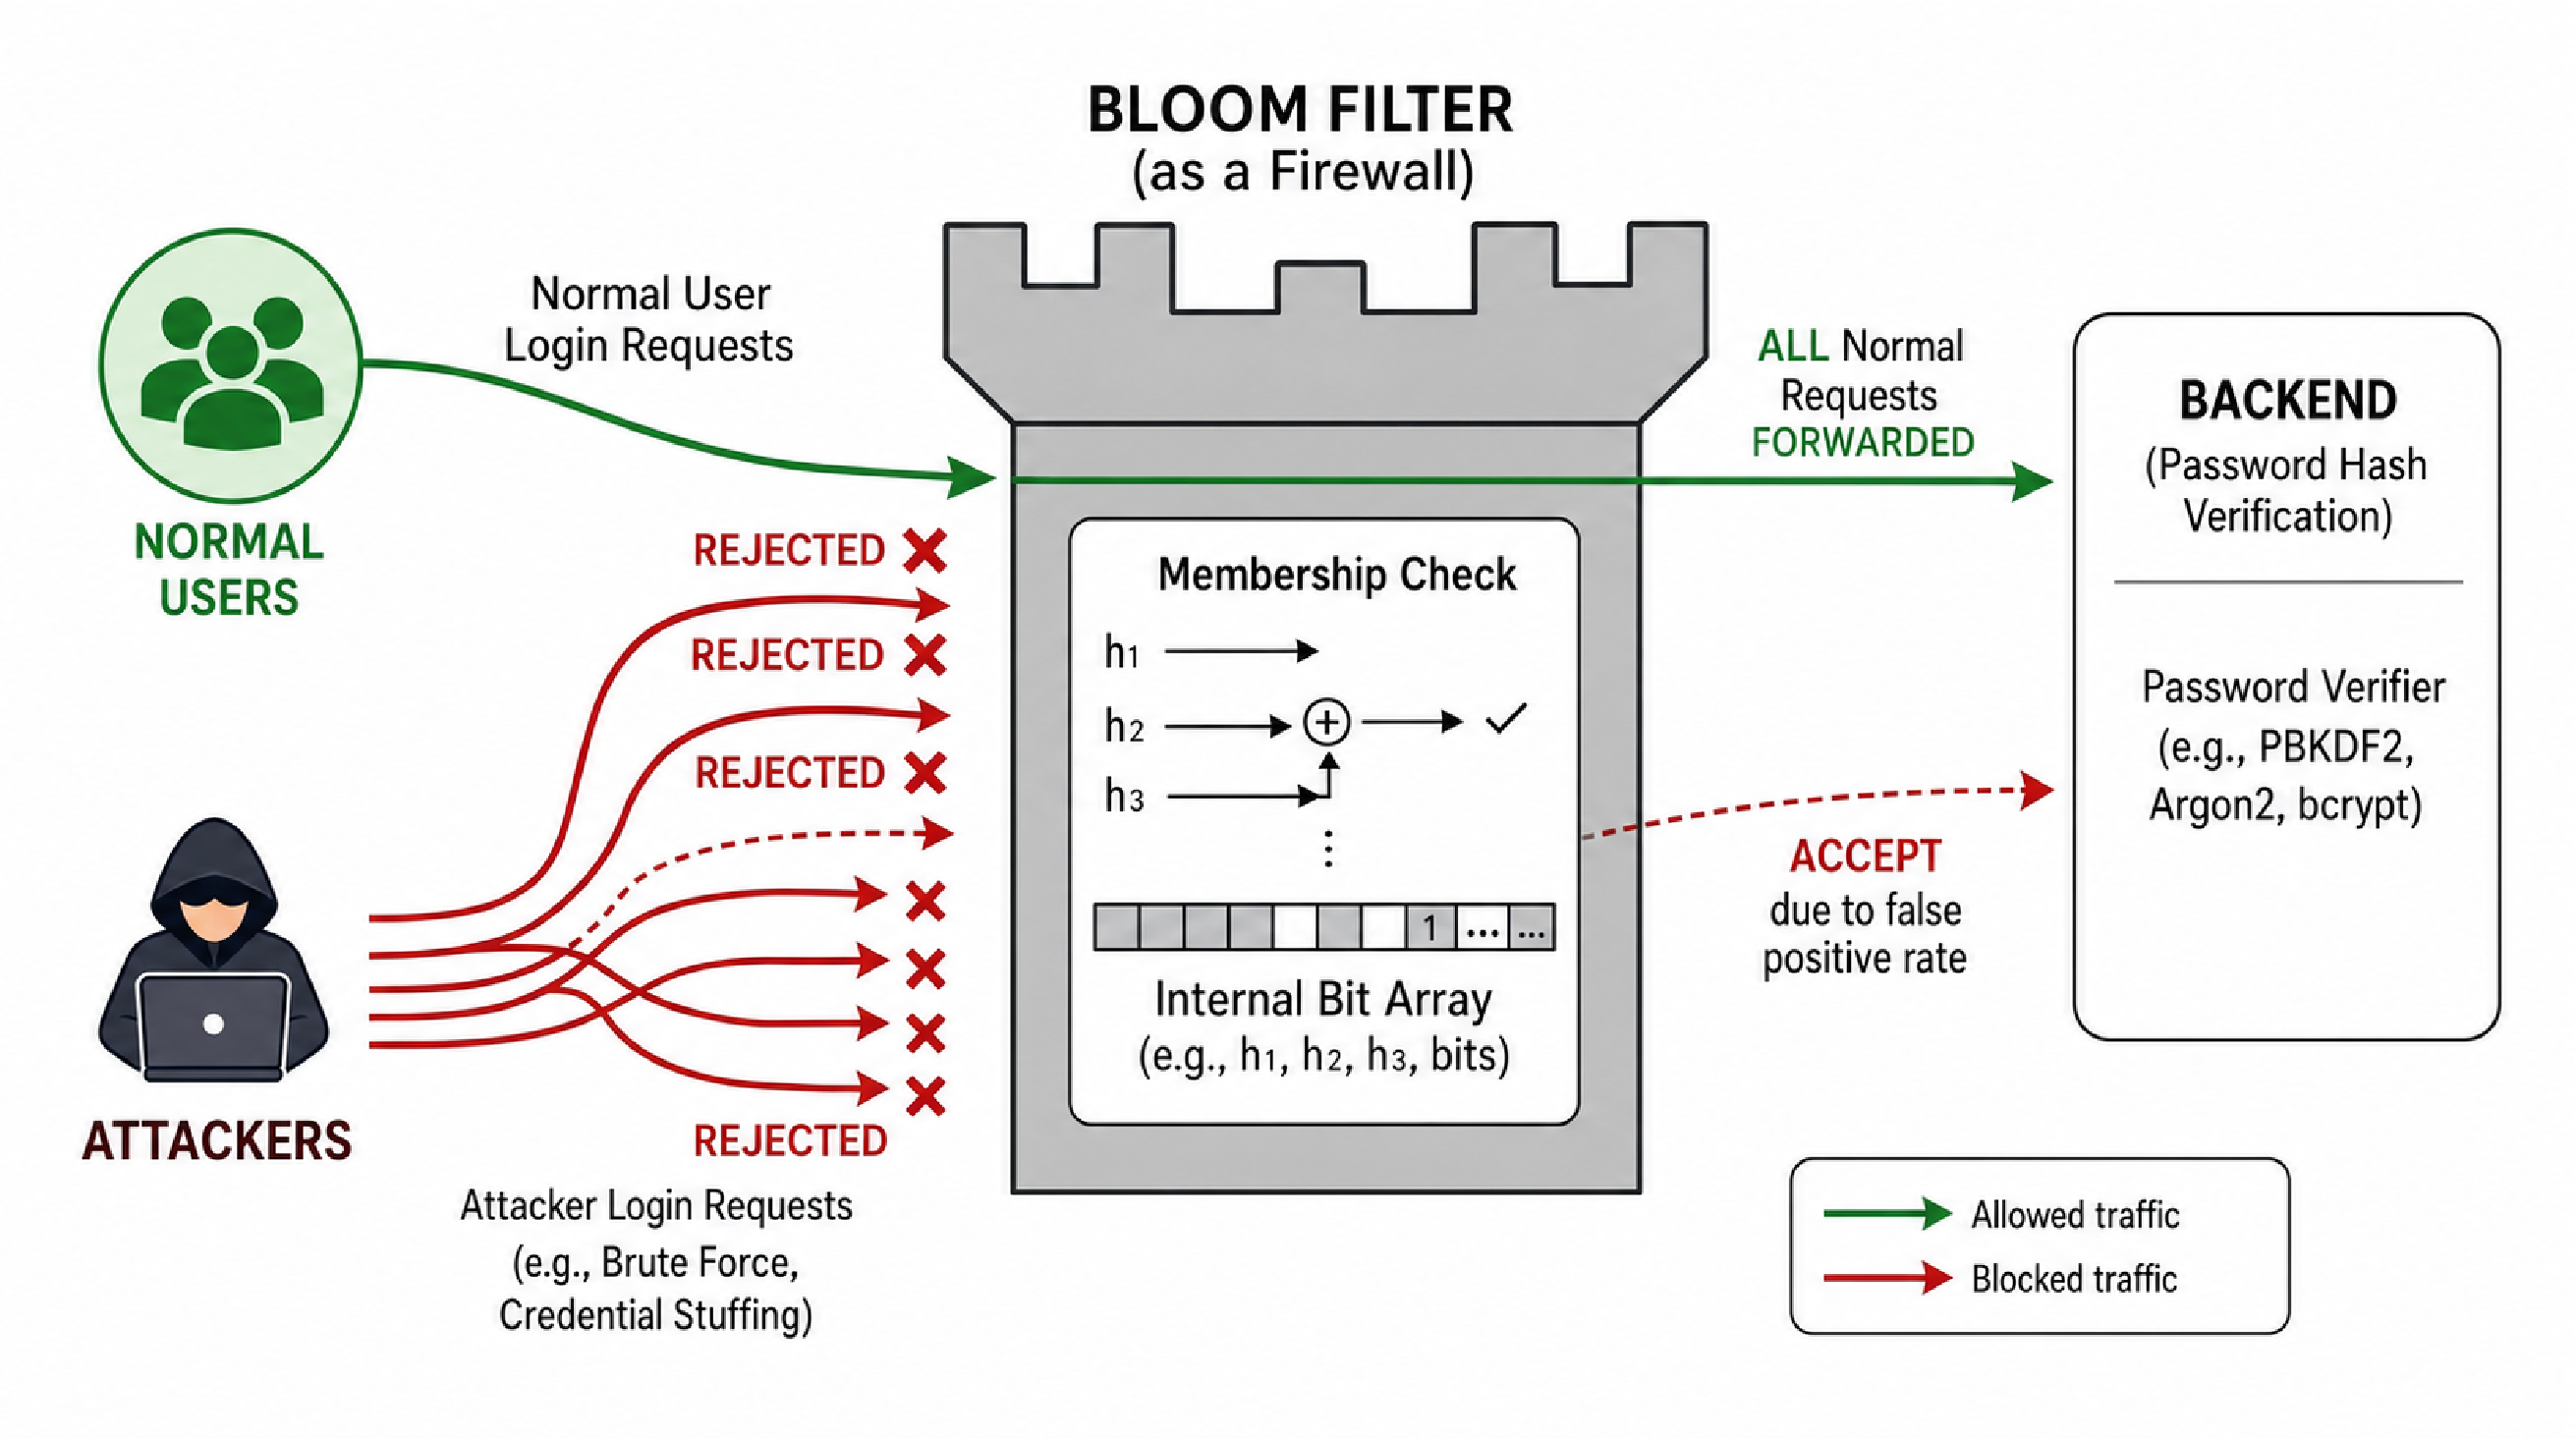
\includegraphics[width=\linewidth]{figure/LBF_pic/new_lbf_fig2.pdf}
  \caption{TRAPS as a one-sided admission-index layer before the password-verification backend.}
  \label{fig:systemoverview}
\end{figure}

TRAPS separates routing, indexing, and authentication. The learning and risk oracle selects a stable region for the submitted credential. The region-local substrate tests whether the corresponding trapdoor is represented. A positive result forwards the request to the backend; it does not authenticate the user. A negative result or replay-cache hit produces the same generic failure response as an ordinary backend reject.

\paragraph{Enrollment and rotation}
When a credential is created or rotated, the backend samples a salt \(s_u\), sets a password-version number \(v_u\), and stores the slow verifier \(H(pw,s_u)\). Registration-time policy may reject passwords using exact policy checks. If a credential is accepted but marked risky, for example due to known-password-list membership or chosen-password registration signals, TRAPS records a stable risk marker and inserts the credential trapdoor into a hardened region.

\paragraph{Login}
For a login attempt \((u,pw)\), the frontend obtains salt, stable metadata, and version from a read-only edge directory. Unknown usernames use a dummy tuple. TRAPS computes the region, derives the trapdoor, checks the replay-suppression cache, and queries the region-local substrate. Only positive, non-cached attempts reach the backend.

\paragraph{Stable route coverage}
For online context \(c\), let \(\Gamma_e(u,pw,c)\) be the set of epoch/region pairs that may contain the current represented credential under the deployment's routing contract. TRAPS may locally reject only after every substrate in \(\Gamma_e\) has been queried and returned negative. The evaluated \texttt{stable\_only} profile makes \(\Gamma_e\) a singleton by using credential- and epoch-stable features. A deployment that uses volatile context such as source, device, or time for region selection must either replicate the credential across all possible queried regions or fail-to-backend rather than AMQ-rejecting when coverage cannot be computed.

\paragraph{Backend feedback}
If the backend returns a definitive credential mismatch for a forwarded request, TRAPS records a replay token for that tuple. Subsequent submissions of the same invalid tuple are rejected before expensive verification.

\subsection{Threat Model}
\label{sec:threat-model}

We consider an online availability adversary whose goal is to maximize the number of incorrect attempts that reach the expensive backend. The adversary may choose usernames and passwords adaptively, distribute requests across many sources, use leaked or popular password lists, and infer from side effects that some invalid requests reached the backend.

The adversary knows the architecture, public algorithms, and broad feature families. Unless explicitly stated otherwise, it does not know epoch trapdoor keys, replay-cache keys, protected screening records, non-public stable metadata, or live indexing state. TRAPS does not rely on secrecy of the learned routing model; Section~\ref{sec:correctness-bound} gives the steering bound when per-region caps are enforced.

\paragraph{Known-password attack}
In a known-password attack, denoted \(\mathsf{KPwA}\), the adversary does not modify the active credential set during the attack window. It issues login attempts whose password distribution is concentrated on known weak, leaked, popular, policy-denied, or otherwise attacker-preferred passwords. Attempts that happen to be correct credentials are forwarded by design and are not counted as pre-screening failures.

Let \(U_j^{(\mathrm{K})}(T)\) be the number of distinct invalid credential tuples routed to region \(j\) during window \([0,T]\), after collapsing exact replays of the same tuple. The expected backend load from first-time invalid false forwards is
\[
\mathbb{E}
\left[
F_{\mathrm{adv}}^{(\mathrm{K})}(T)
\right]
=
\sum_{j=1}^{r}
U_j^{(\mathrm{K})}(T)\varepsilon_j.
\]

\paragraph{Chosen-password attack}
In a chosen-password attack, denoted \(\mathsf{CPwA}\), the adversary obtains bounded access to normal registration, password-reset, or password-rotation interfaces. Each successful operation creates or changes an attacker-controlled credential and causes a pre-verifier insertion. These operations are subject to the service's ordinary abuse controls and have non-negligible cost.

Let \(\Delta_j\) be the number of attacker-chosen accepted credentials inserted into region \(j\). If the occupancy of region \(j\) changes from \(N_j\) to
\[
N_j'=N_j+\Delta_j,
\]
then a subsequent invalid flood with \(U_j^{(\mathrm{C})}(T)\) distinct invalid tuples has expected residual backend load
\[
\mathbb{E}
\left[
F_{\mathrm{adv}}^{(\mathrm{C})}(T)
\right]
=
\sum_{j=1}^{r}
U_j^{(\mathrm{C})}(T)\varepsilon_j(N_j+\Delta_j).
\]
This models indexing-state poisoning and false-forward amplification. Successful logins using attacker-owned valid credentials remain ordinary valid traffic and are handled by complementary account-abuse controls.

\paragraph{Backend-overload objective}
Let \(C_{\mathrm{BE}}\) be the sustained backend capacity in full password verifications per unit time. Let \(L_{\mathrm{hon}}(T)\) be honest forwarded load and \(F_{\mathrm{adv}}(T)\) be attacker-induced false-forwarded load. The backend is overloaded if
\[
L_{\mathrm{hon}}(T)+F_{\mathrm{adv}}(T)\ge C_{\mathrm{BE}}T.
\]
TRAPS improves availability by reducing \(F_{\mathrm{adv}}(T)\) through region-specific residual budgets and replay suppression.

\paragraph{Out of scope}
TRAPS targets the password-verifier bottleneck under invalid-credential pressure. Attacks consisting solely of repeated logins using already-valid attacker-owned credentials are handled by complementary controls such as registration throttling, CAPTCHA, proof-of-work, payment or identity friction, per-account rate limits, and risk-based step-up authentication. Network-layer flooding, connection exhaustion, full compromise of the trusted first-party frontend, and post-compromise offline password cracking using exposed screening keys and indexing state are outside the core availability claim.

\paragraph{Username enumeration}
Unknown usernames follow a dummy-salt and dummy-metadata path, and local drops and backend rejects use the same generic failure response. TRAPS is designed not to introduce a semantic username-enumeration channel beyond that of the underlying service. Operational deployments should additionally equalize directory hit and miss behavior, avoid branch-specific errors, rate-limit repeated probes, and monitor timing distributions for distinguishers.

\paragraph{Deployment failure modes}
The one-sided guarantee is conditional on operational invariants rather than on the learned model. A stale edge directory can route a newly active credential before its trapdoor is represented, so activation must be atomic or fail-to-backend until backend-only verification is safe. Replay-cache entries must be exact, versioned, and inserted only after definitive backend mismatches; approximate negative caches or stale password-version entries can create false rejects. Migration crashes are handled by keeping the old epoch queryable until the new epoch is fully populated and durably activated. Stale Bloom bits after password rotation only increase false forwards and are removed by rebuild or dynamic AMQ maintenance. Trapdoor and replay keys are rotated by epoch with dual-query migration; key compromise or full frontend compromise is outside the core claim and requires emergency rebuild and backend-side abuse controls. Timing padding and dummy-directory behavior are required when username enumeration resistance is part of the deployment objective.
